\section{Ruch kamery}

\subsection{Pozycja kamery}

    Widok w grze jest trzecioosobowy, kamera obejmuje zarówno widzialny obszar jak i samego gracza. Pod tym względem jest to gra TPP (\textit{Third Person Perspective}). Przykładowymi grami tego typu są bardzo znane produkcje, takie jak seria \textit{Wiedźmin}, \textit{Tomb Raider}, czy \textit{GTA}.

    Aby uzyskać efekt kamery podążającej za graczem, obiekt kamery powinien zostać umieszczony wewnątrz obiektu gracza w hierarchii obiektów. W ten sposób koordynacje kamery będą ustawiane względem gracza, a sama kamera poruszać się będzie i obracać wraz z nadrzędnym obiektem.

    Koordynacje kamery ustawiliśmy na (0, 0, 0), w ten sposób kamera jest w środkowym punkcie obiektu nadrzędnego i wytarczy za pomocą narzędzi transformacji przesunąć ją do oczekiwanej pozycji (tak, aby obejmowała obraz zza pleców postaci). Inną, bardziej poręczną metodą jest odpowiednie dostosowanie widoku sceny i skopiowanie jego koordynatów do zaznaczonej w hierarchii kamery.

    \begin{figure}[H]
    \center
    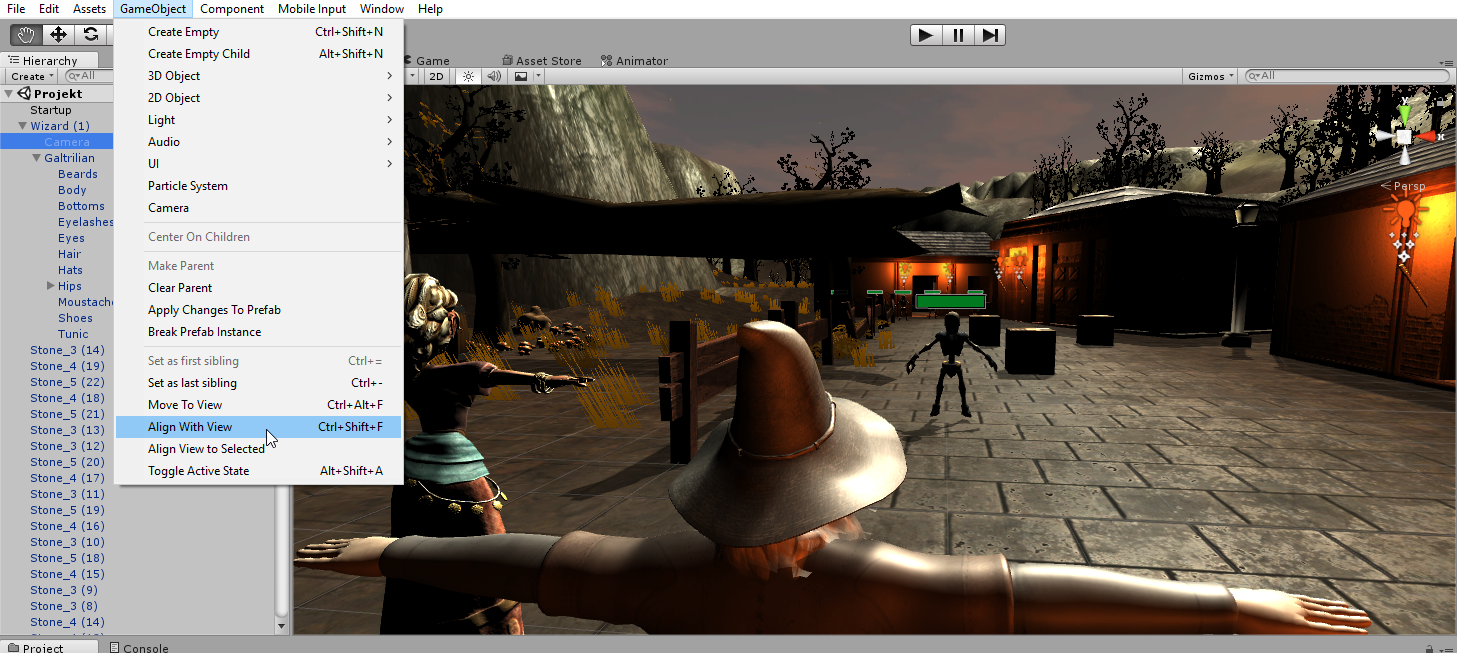
\includegraphics[width=\textwidth]{kamera_1.png}
    \caption{Dostosowanie pozycji kamery gracza względem aktualnego widoku sceny}
    \end{figure}

\subsection{Mechanika obrotu kamery}

Kolejnym etapem jest oprogramowanie ruchu kamery za pomocą ruchów myszy. Mysz jest używana również do obrotu postacią. Jako, że kamera \enquote{przyklejona} jest do postaci, aby uzyskać efekt rozglądania się, modyfikujemy jedynie jej obrót w pionie, natomiast ruch myszy w poziomie obraca poziomo całą postać wraz z kamerą.

\begin{figure}[H]
\center
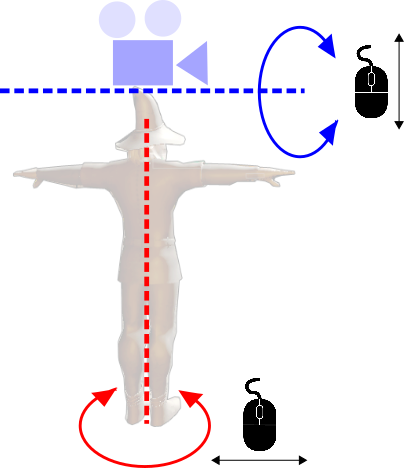
\includegraphics[width=9cm]{kamera_2.png}
\caption{Schemat działania systemu sterowania kamerą}
\end{figure}

\begin{lstlisting}[caption={Obrót kamery za pomocą myszy}]
if (!photonView.isMine) return;
if (!stopCamera)
{
    Camera.main.transform.Rotate(new Vector3(-Input.GetAxis("Mouse Y") * rotationSensitivity * Time.deltaTime, 0, 0));
    rb.transform.Rotate(new Vector3(0, Input.GetAxis("Mouse X") * rotationSensitivity * Time.deltaTime, 0));
}
\end{lstlisting}

Obrót kamery polega na dodaniu wektora obrotu do odpowiedniej osi kamery, natomiast wielkość wektora określona jest przez wartość chwilowego przesunięcia myszy, skalowanego parametrem \textit{rotationSensivity} w celu określenia czułości myszki. Parametr \textit{Time.deltaTime} zwraca czas od ostatniej wyrenderowanej klatki, co pozwala na uzyskanie jednolitej czułości myszki bez względu na ilość generowanych klatek na sekundę.

\subsection{Celownik}

Aby ułatwić celowanie w przeciwników oraz interakcję z otoczeniem umieściliśmy w grze celownik, który w dalszym etapie tworzenia gry zmienia kolor informując o możliwej interakcji.

Celownik jest obiektem 2D nałożonym na ekran w formie \textit{Sprite'a}. Sprite'y to 2-wymiarowe, wcześniej przygotowane obiekty graficzne. W naszym wypadku posłużyliśmy się bezstratnym formatem PNG.

Do sceny został dodany obiekt, na który nałożyliśmy komponenty \name{Canvas} oraz \name{CanvasScaler}. Nakładają one na ekran dwuwymiarowe płótno oraz pozwalają na skalowane go względem podanej rozdzielczości referencyjnej. Wewnątrz takiego płótna można umieszczać obrazy, elementy interfejsu oraz różnego rodzaju wskaźniki (np. Pasek postępu życia bohatera).

\begin{figure}[H]
\center
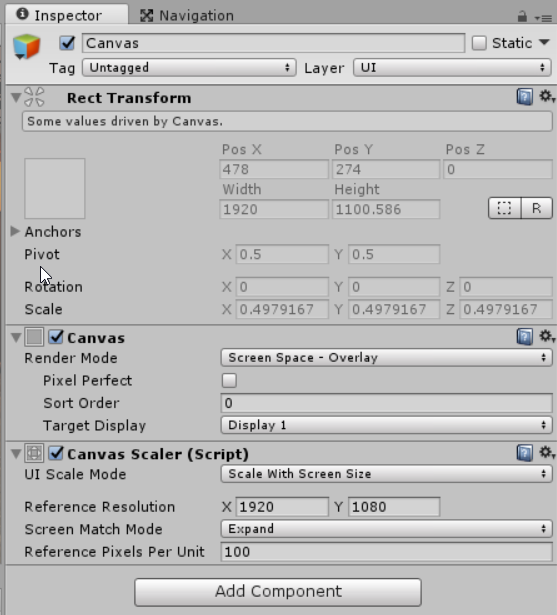
\includegraphics[width=5cm]{celownik_1.png}
\caption{Konfiguracja płutna 2D do wyświetlania interfejsu gry}
\end{figure}

Wewnątrz płótna został umieszczony obrazek (komponent \name{Image}) celownika, wyrównany do środka ekranu.

\begin{figure}[H]
\center
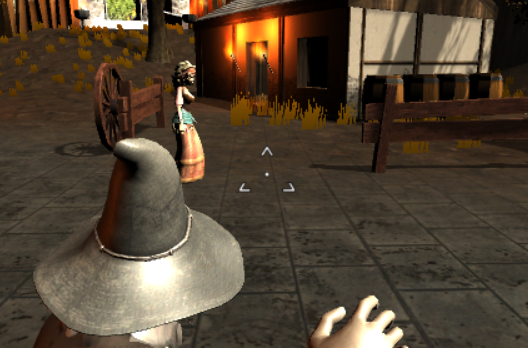
\includegraphics[width=6cm]{celownik_2.png}
\caption{Gotowy celownik gracza}
\end{figure}